% Figura 6: Arquitectura del Transformer GLM-4.7 con intervención
% Muestra dónde se aplica la orthogonalización y el kernel Gaussiano
%
% Compilar con: pdflatex fig6_transformer_architecture.tex
%
\documentclass[12pt]{article}
\usepackage[paperwidth=22cm,paperheight=18cm,margin=0.5cm]{geometry}
\usepackage{tikz}
\usepackage{amsmath}
\pagestyle{empty}
\usetikzlibrary{arrows.meta, calc, decorations.pathreplacing, positioning, shapes.geometric, fit, backgrounds}

% Colores
\definecolor{embedcolor}{RGB}{31,119,180}
\definecolor{attncolor}{RGB}{214,39,40}
\definecolor{mlpcolor}{RGB}{44,160,44}
\definecolor{moecolor}{RGB}{255,127,14}
\definecolor{normcolor}{RGB}{148,103,189}
\definecolor{kernelcolor}{RGB}{23,190,207}
\definecolor{optimalcolor}{RGB}{227,119,194}

\begin{document}
\centering
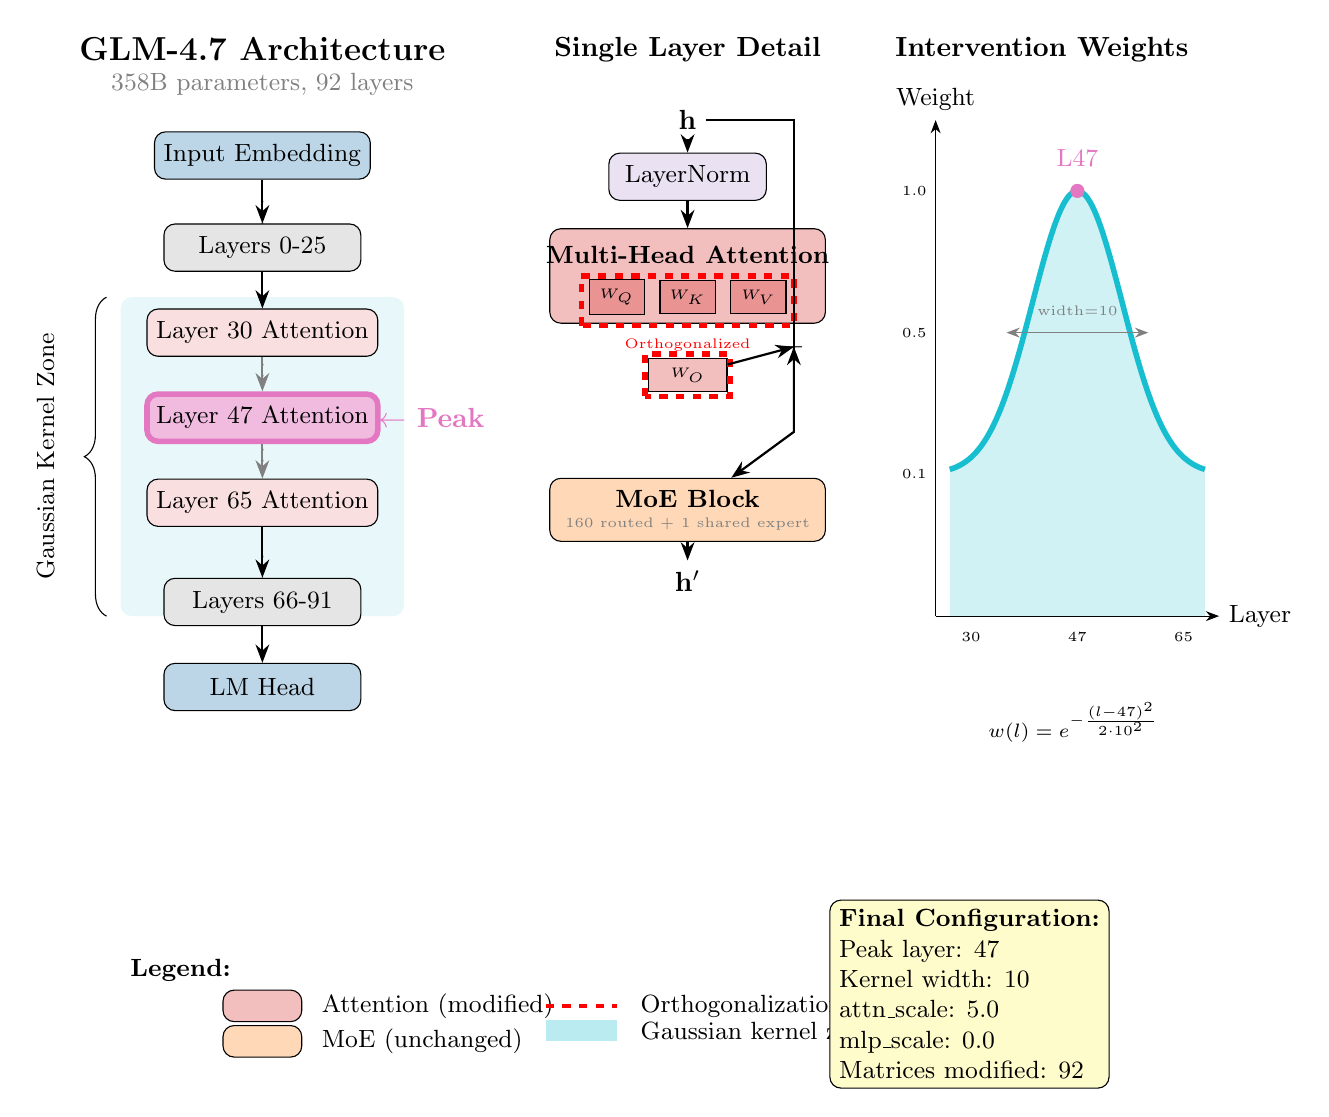
\begin{tikzpicture}[
    scale=0.9,
    >=Stealth,
    layer/.style={draw, rounded corners, minimum width=2.5cm, minimum height=0.6cm, font=\small},
    attn/.style={layer, fill=attncolor!30},
    mlp/.style={layer, fill=mlpcolor!30},
    moe/.style={layer, fill=moecolor!30},
    norm/.style={layer, fill=normcolor!20, minimum width=2cm},
    embed/.style={layer, fill=embedcolor!30},
    intervention/.style={draw=red, line width=2pt, dashed},
]

% === COLUMNA IZQUIERDA: Arquitectura del Modelo ===
\begin{scope}[shift={(-4,0)}]
    % Título
    \node[font=\bfseries\large] at (0,10) {GLM-4.7 Architecture};
    \node[font=\small, gray] at (0,9.5) {358B parameters, 92 layers};

    % Input
    \node[embed] (input) at (0,8.5) {Input Embedding};

    % Capas tempranas (comprimidas)
    \node[font=\small, gray] at (0,7.8) {$\vdots$};
    \node[layer, fill=gray!20] (early) at (0,7.2) {Layers 0-25};

    % Zona de intervención
    \begin{scope}[on background layer]
        \fill[kernelcolor!10, rounded corners] (-2,6.5) rectangle (2,2);
    \end{scope}

    % Kernel zone label
    \draw[decorate, decoration={brace, amplitude=8pt, mirror}] (-2.2,6.5) -- (-2.2,2);
    \node[font=\small, rotate=90, anchor=south] at (-2.8,4.25) {Gaussian Kernel Zone};

    % Capas con intervención
    \node[attn, fill=attncolor!15] (l30) at (0,6) {Layer 30 Attention};
    \node[font=\small, gray] at (0,5.5) {$\vdots$};

    % Capa 47 (óptima) - destacada
    \node[attn, fill=optimalcolor!50, line width=2pt, draw=optimalcolor] (l47) at (0,4.8) {Layer 47 Attention};
    \node[font=\bfseries, optimalcolor, anchor=west] at (1.5,4.8) {$\leftarrow$ Peak};

    \node[font=\small, gray] at (0,4.3) {$\vdots$};
    \node[attn, fill=attncolor!15] (l65) at (0,3.6) {Layer 65 Attention};

    % Capas tardías
    \node[font=\small, gray] at (0,2.8) {$\vdots$};
    \node[layer, fill=gray!20] (late) at (0,2.2) {Layers 66-91};

    % Output
    \node[embed] (output) at (0,1) {LM Head};

    % Flechas de flujo
    \draw[->, thick] (input) -- (early);
    \draw[->, thick] (early) -- (l30);
    \draw[->, thick, gray] (l30) -- (l47);
    \draw[->, thick, gray] (l47) -- (l65);
    \draw[->, thick] (l65) -- (late);
    \draw[->, thick] (late) -- (output);

\end{scope}

% === COLUMNA CENTRAL: Detalle de una capa ===
\begin{scope}[shift={(2,4)}]
    % Título
    \node[font=\bfseries] at (0,6) {Single Layer Detail};

    % Input
    \node (lin) at (0,5) {$\mathbf{h}$};

    % LayerNorm
    \node[norm] (norm1) at (0,4.2) {LayerNorm};

    % Multi-Head Attention (expandido)
    \begin{scope}[shift={(0,2.8)}]
        \node[attn, minimum width=3.5cm, minimum height=1.2cm] (mha) at (0,0) {};
        \node[font=\small\bfseries] at (0,0.3) {Multi-Head Attention};

        % Q, K, V matrices
        \node[draw, fill=attncolor!50, minimum width=0.7cm, minimum height=0.4cm, font=\tiny] (wq) at (-1,-.3) {$W_Q$};
        \node[draw, fill=attncolor!50, minimum width=0.7cm, minimum height=0.4cm, font=\tiny] (wk) at (0,-.3) {$W_K$};
        \node[draw, fill=attncolor!50, minimum width=0.7cm, minimum height=0.4cm, font=\tiny] (wv) at (1,-.3) {$W_V$};

        % Intervention markers
        \draw[intervention] (-1.5,-0.7) rectangle (1.5,0);
        \node[font=\tiny, red, anchor=north] at (0,-0.75) {Orthogonalized};
    \end{scope}

    % Output projection
    \node[draw, fill=attncolor!30, minimum width=1cm, font=\tiny] (wo) at (0,1.4) {$W_O$};
    \draw[intervention] (-0.6,1.1) rectangle (0.6,1.7);

    % Add & Norm
    \node[font=\small] at (1.5,1.8) {$+$};
    \draw[->, thick] (lin) -- ++(1.5,0) |- (1.5,1.8);
    \draw[->, thick] (wo) -- (1.5,1.8);

    % MoE Block
    \begin{scope}[shift={(0,-0.5)}]
        \node[moe, minimum width=3.5cm, minimum height=0.8cm] (moe) at (0,0) {};
        \node[font=\small\bfseries] at (0,0.15) {MoE Block};
        \node[font=\tiny, gray] at (0,-0.2) {160 routed + 1 shared expert};
    \end{scope}

    % Output
    \node (lout) at (0,-1.5) {$\mathbf{h}'$};

    % Arrows
    \draw[->, thick] (lin) -- (norm1);
    \draw[->, thick] (norm1) -- (mha);
    \draw[->, thick] (1.5,1.8) -- ++(0,-1.2) -- (moe);
    \draw[->, thick] (moe) -- (lout);

\end{scope}

% === COLUMNA DERECHA: Kernel Gaussiano ===
\begin{scope}[shift={(7,4)}]
    % Título
    \node[font=\bfseries] at (0,6) {Intervention Weights};

    % Ejes
    \draw[->] (-1.5,-2) -- (-1.5,5) node[above, font=\small] {Weight};
    \draw[->] (-1.5,-2) -- (2.5,-2) node[right, font=\small] {Layer};

    % Curva Gaussiana
    \draw[kernelcolor, line width=2pt, smooth] plot[domain=-1.3:2.3, samples=50]
        (\x, {4*exp(-(\x-0.5)^2/0.8)});
    \fill[kernelcolor, opacity=0.2] plot[domain=-1.3:2.3, samples=50]
        (\x, {4*exp(-(\x-0.5)^2/0.8)}) -- (2.3,-2) -- (-1.3,-2) -- cycle;

    % Peak marker
    \fill[optimalcolor] (0.5,4) circle (0.1);
    \node[font=\small, optimalcolor, anchor=south] at (0.5,4.2) {L47};

    % Layer labels
    \node[font=\tiny] at (-1,-2.3) {30};
    \node[font=\tiny] at (0.5,-2.3) {47};
    \node[font=\tiny] at (2,-2.3) {65};

    % Weight values
    \node[font=\tiny] at (-1.8,4) {1.0};
    \node[font=\tiny] at (-1.8,2) {0.5};
    \node[font=\tiny] at (-1.8,0) {0.1};

    % FWHM
    \draw[<->, gray] (-0.5,2) -- (1.5,2);
    \node[font=\tiny, gray, anchor=south] at (0.5,2.1) {width=10};

    % Fórmula
    \node[font=\scriptsize, align=center] at (0.5,-3.5) {
        $w(l) = e^{-\frac{(l-47)^2}{2 \cdot 10^2}}$
    };
\end{scope}

% === LEYENDA ===
\begin{scope}[shift={(-4,-3)}]
    \node[font=\bfseries\small, anchor=west] at (-2,0) {Legend:};

    \node[attn, minimum width=1cm, minimum height=0.4cm] at (0,-0.5) {};
    \node[font=\small, anchor=west] at (0.7,-0.5) {Attention (modified)};

    \node[moe, minimum width=1cm, minimum height=0.4cm] at (0,-1) {};
    \node[font=\small, anchor=west] at (0.7,-1) {MoE (unchanged)};

    \draw[intervention, line width=1.5pt] (4,-0.5) -- (5,-0.5);
    \node[font=\small, anchor=west] at (5.2,-0.5) {Orthogonalization applied};

    \fill[kernelcolor!30] (4,-1) rectangle (5,-0.7);
    \node[font=\small, anchor=west] at (5.2,-0.85) {Gaussian kernel zone};
\end{scope}

% === CONFIGURACIÓN FINAL ===
\node[draw, rounded corners, fill=yellow!20, font=\small, align=left, anchor=north west] at (4,-2) {
    \textbf{Final Configuration:}\\
    Peak layer: 47\\
    Kernel width: 10\\
    attn\_scale: 5.0\\
    mlp\_scale: 0.0\\
    Matrices modified: 92
};

\end{tikzpicture}
\end{document}
